\documentclass{article}

\usepackage[utf8]{inputenc}
\usepackage[T1]{fontenc}
\usepackage{amsmath}
\usepackage{amsfonts}
\usepackage{amssymb}
\usepackage[version=4]{mhchem}
\usepackage{stmaryrd}
\usepackage{bbold}
\usepackage{graphicx}
\usepackage{adjustbox}
\usepackage{tocloft}   % For TOC formatting
\usepackage{geometry}  % For margins
\usepackage{titlesec}  % For section formatting
\usepackage{fancyhdr}
\usepackage{float}
\usepackage[stable]{footmisc}
\usepackage{hyperref}  % For clickable links in TOC (load last)
\usepackage{mdframed}  
\usepackage{listings}  



% Document styling
\geometry{margin=1in}

% Customize section formatting (option 2: let titlesec handle the label)
\titleformat{\section}
  {\normalfont\Large\bfseries} % format
  {\thesection}                % label
  {0.5em}                      % separation
  {\rule{\textwidth}{0.4pt}\vspace{0.5em}\newline} % before-code

% adding a header
\pagestyle{fancy}
\fancyhf{}
\lhead{Problem Set 4}
\rhead{Henrik Berger - Romain Fernex}
\cfoot{ \thepage}
\renewcommand{\headrulewidth}{0.8pt}

\title{Problem Set 4 - Macroeconomics}
\author{Henrik Berger - Romain Fernex}
\date{February 2025}

\begin{document}

\maketitle
\tableofcontents
\newpage

\section{Literature review}

\begin{figure}[H]
    \centering
    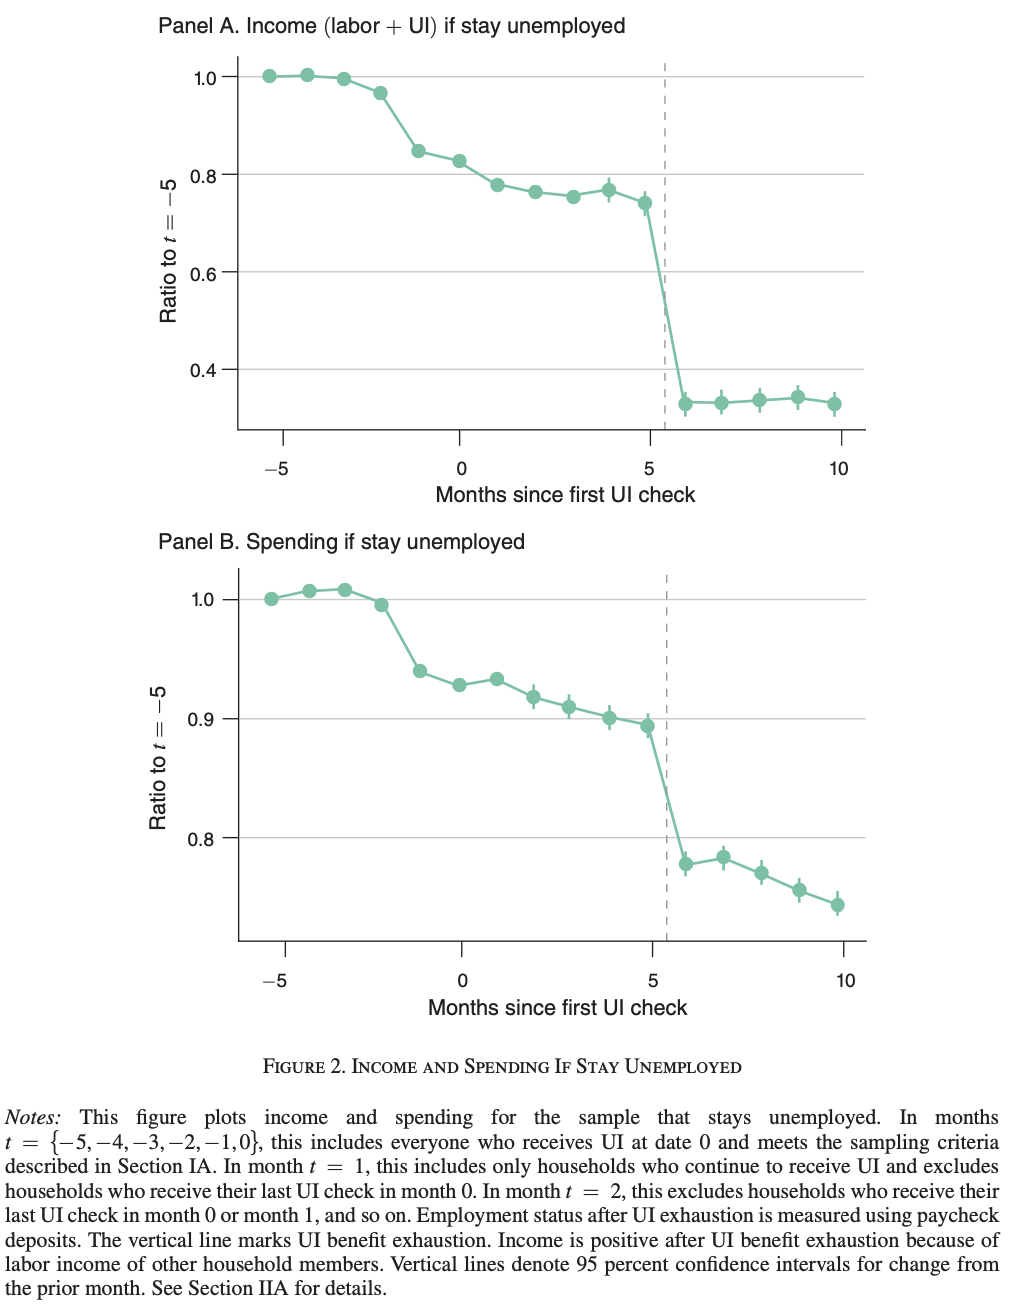
\includegraphics[width=0.8\textwidth]{figures/Screenshot 2025-11-11 at 2.41.56 PM.png}
    \caption{Evolution of household spendings in response to unemployment shock}
    \label{fig: unemployment and MPC}
\end{figure}

The figure from Ganong and Noel (AER, 2019, Figure 2) follows income and spending for households that remain unemployed through UI exhaustion. Income, normalized to month -5, declines gradually from about 1.0 to 0.85 by month 5 and then drops sharply to roughly 0.45 at the moment benefits expire, a fully predictable change. Spending also falls gradually during unemployment but shows a clear additional decline at exhaustion, from around 0.90 to about 0.82. The fact that spending decreases discretely when the income loss is anticipated contradicts the permanent income hypothesis, which predicts smooth consumption in the face of predictable shocks. Instead, it implies a high marginal propensity to consume (MPC) out of UI benefits, consistent with households having limited liquidity or insufficient buffer assets. The magnitude is economically meaningful: a roughly 40\% income drop generates about an 8\% spending drop, suggesting MPCs far above zero and strong dependence on UI for maintaining consumption. The gradual decline before exhaustion indicates partial anticipation, but the discontinuity shows that forward-looking adjustments cannot fully offset constraints. Overall, the figure highlights that UI benefits play a central role in consumption smoothing and that extending benefit duration may significantly reduce consumption volatility during long unemployment spells.

\section{Exercise I}
\subsection{1)}
We denote $s^t$ the history of the states of the world at time t and $s_t$ the state of the world at time t. 
We have the following expression tying $\pi_t(s^t)$ to $\pi_0(s^0)$, with $s^0$ the state of the world at time $0$ (initialization period) :
$$\pi_t(s^t)=\pi_0(s^0)\prod_{i=0}^{t-1}\pi_i(s^{i+1}|s^i)$$

\subsection{2)}
The planner's problem is as follows : 
$$\begin{aligned}
    &\max_{\{c_1^t(s^t),c_2^t(s^t)\}_{\forall t,s^t\in S^t}}\theta \sum_{t=0}^\infty\sum_{s^t\in S^t}\beta^tln(c_1^t(s^t))\pi_t(s^t)+(1-\theta)\sum_{t=0}^\infty\sum_{s^t\in S^t}\beta^tln(c_2^t(s^t))\pi_t(s^t)\\
    &\text{s.t} \quad c_1^t(s^t)+c_2^t(s^t)=y_1^t+y_2^t=s_t+1 \quad \forall t,s^t\in S^T
\end{aligned}$$
We can write the Lagrangian for this problem : we denote $\lambda_t(s^t)$ the shadow value for each $t,s^t$
$$\begin{aligned}\mathcal{L}= &\theta \sum_{t=0}^\infty\sum_{s^t\in S^t}\beta^tln(c_1^t(s^t))\pi_t(s^t)+(1-\theta)\sum_{t=0}^\infty\sum_{s^t\in S^t}\beta^tln(c_2^t(s^t))\pi_t(s^t)\\
&+\sum_{t=0}^\infty\sum_{s^t\in S^t}\lambda _t(s^t)[s^t+1-c_1^t(s^t)-c_2^t(s^t)]
\end{aligned} $$
Let's write down the FOC in $c_1^t(s^t), c_2^t(s^t)$ for any given $t,s^t$
$$\begin{aligned}
    &\text{in }c_1^t(s^t):\quad \theta \beta ^t\frac{\pi_t(s^t)}{c_1^t(s^t)}=\lambda_t(s^t)\\
    &\text{in }c_2^t(s^t):\quad (1-\theta) \beta ^t\frac{\pi_t(s^t)}{c_2^t(s^t)}=\lambda_t(s^t)
\end{aligned}$$
Hence, 
$$\begin{aligned}\theta \beta ^t\frac{\pi_t(s^t)}{c_1^t(s^t)} &= (1-\theta) \beta ^t\frac{\pi_t(s^t)}{c_2^t(s^t)}\\
\Leftrightarrow \theta c_2^t(s^t)&=(1-\theta)c_1^t(s^t)\\
\Leftrightarrow c_2^t(s^t)&=\frac{1-\theta}{\theta}c_1^t(s^t)
\end{aligned}$$
Then, using the aggregate feasibility constraint : 
$$\begin{aligned}
    c_1^t(s^t)+\frac{1-\theta}{\theta}c_1^t(s^t)=s_t+1\\
    \Leftrightarrow c_1^t(s^t)=\theta (s_t+1)
\end{aligned}$$
This gives us : 
$$\left\{\begin{aligned}
   &c_1^t(s^t)=\theta(s_t+1)\\
   &c_2^t(s^t)=(1-\theta)(s_t+1)
\end{aligned} \right.$$
At optimality, each agent gets exactly his pareto weight share of the aggregate endowment for each period and in each possible state 

\subsection{3)}
We denote $q_t^0(s^t)$ the price of the arrow security contingent on state $s^t$. We index it by $0$ as every arrow security is traded at time $0$. 
We now have the following set up for the competitive equilibrium problem : for each agent $i\in \{1,2 \}$
$$\begin{aligned}
    &\max_{c_i^t(s^t)}\sum_{t=0}^\infty \sum_{s^t\in S^t}\beta^t \pi_t(s^t)ln(c_i^t(s^t))\\
    \text{s.t} \quad &\sum_{t=0}^\infty\sum_{s^t\in S^t}q_t^0(s^t)y_i^t(s^t)\geq  \sum_{t=0}^\infty\sum_{s^t\in S^t} q_t^0(s^t)c_i^t(s^t)\quad (\text{resource constraint})
\end{aligned}$$
Then the aggregate feasibility constraint gives us : $$c_1^t(s^t)+c_2^t(s^t)=s_t+1 \quad \forall t,s^t\in S^t $$
For agent 1 the resource constraint is as follows : 
$$\sum_{t=0}^\infty\sum_{s^t\in S^t}q_t^0(s^t)s^t\geq  \sum_{t=0}^\infty\sum_{s^t\in S^t} q_t^0(s^t)c_1^t(s^t)$$
And for agent 2 : 
$$\sum_{t=0}^\infty\sum_{s^t\in S^t}q_t^0(s^t)\geq  \sum_{t=0}^\infty\sum_{s^t\in S^t} q_t^0(s^t)c_2^t(s^t)$$

\subsection{4)}
Now, let's solve for equilibrium prices : first, we write the lagrangian for any $i\in \{1,2\}$
$$\mathcal{L}=\sum_{t=0}^\infty\sum_{s^t\in S^t}\beta^t\pi_t(s^t)ln(c_i^t(s^t))+\lambda_i\sum_{t=0}^\infty\sum_{s^t\in S^t}q_t^0(s^t)[y_i^t(s^t)-c_i^t(s^t)]$$
As we did for Pareto, we take the FOC in $c_i^t{(s^t)}$ : 
$$\frac{\beta^t\pi_t(s^t)}{c_i^t(s^t)}=\lambda_i q_t^0(s^t) \quad \forall t,i,s^t\in S^t$$
Then, taking the ratio of the FOC for each agent : 
$$\frac{\beta^t\pi_t(s^t)c_2^t(s^t)}{\beta^t\pi_t(s^t)c_1^t(s^t)}=\frac{\lambda_1q_t^0(s^t)}{\lambda_2q_t^0(s^t)}\Leftrightarrow c_2^t(s^t) =\frac{\lambda_1}{\lambda_2}c_1^t(s^t)$$
Then, using the aggregate feasibility constraint : 
$$\left\{\begin{aligned}
    c_1^t(s^t)(1+\frac{\lambda_1}{\lambda_2})=s_t+1\\
    c_2^t(s^t)(1+\frac{\lambda_2}{\lambda_1})=s_t+1
\end{aligned} \right.$$
Lastly, let's replace consumption in the FOC using the above and compute equilibrium prices as a function of the shadow values : 
$$\begin{aligned}
    \left\{\begin{aligned}
        \frac{1}{\lambda_1}\frac{\beta^t\pi_t(s^t)}{s^t+1}\frac{\lambda_2+\lambda_1}{\lambda_2} = q_t^0(s^t)\\
        \frac{1}{\lambda_2}\frac{\beta^t\pi_t (s^t)}{s^t+1}\frac{\lambda_1+\lambda_2}{\lambda_1}=q_t^0(s^t)
    \end{aligned} \right.\\
    \Leftrightarrow q_t^0(s^t) = \frac{\beta^t\pi_t(s^t)}{s_t+1}(\frac{1}{\lambda_1}+\frac{1}{\lambda_2})
\end{aligned}$$

\subsection{5)}
Based on the results we got in (2) and (5), we have : 
$$\begin{aligned}
    \text{Pareto : }\left\{\begin{aligned} &c_1^t(s^t) = \theta (s_t+1)\\
    &c_2^t(s^t)=(1-\theta)(s_t+1)
    \end{aligned}\right.\\
    \text{Competitive : } \left\{\begin{aligned} &c_1^t(s^t) = \frac{\lambda_2}{\lambda_1+\lambda_2} (s_t+1)\\
    &c_2^t(s^t)=\frac{\lambda_1}{\lambda_1+\lambda_2}(s^t+1)
    \end{aligned}\right.
\end{aligned}$$
The two solutions coincide when : 
$$\lambda_1 \propto 1-\theta \quad \text{and} \quad \lambda_2\propto \theta$$
This is in line with the First Welfare Theorem : every Pareto-efficient allocation (with weights $\theta,1-\theta\in]0,1[)$ can be decentralized as a competitive equilibrium by choosing household wealth (or transfers) so that the resulting budget multipliers satisfy the ratio above. Then the induced Arrow-Debreux prices support that allocation

 
\section{Exercise II}

Link to the Notebook with the Julia code for the full Aiyagari : \href{https://pluto.land/n/mugr1ub9}{Notebook for Exercise 2} 

\section{Reference}
Ganong, Peter, and Pascal Noel. 2019. "Consumer Spending during Unemployment: Positive and Normative Implications." American Economic Review 109 (7): 2383–2424.

\end{document}


